\section{Semana 3 - Mission Profile + MTOW Estimation}
\subsection{Introdução}
Nesta secção, apresenta-se a missão bem definida da nossa aeronave bem como o Maximum Take Off Weight (MTOW).\par
Nesta semana foi introduzido um programa escrito em Matlab fornecido aos alunos. Este possibilita o cálculo do design point bem como a estimação de múltiplos parâmetros baseado em equações de desempenho e valores empíricos. A falta de documentação do programa e de comentários no source code levou a que certas funcionalidades e dados não tinham sido utilizados imediatamente, dado terem sido encontrados posteriormente. Além de tal, limitações do programa bem como a inexistência de equações empíricas para certos designs limitou a escolha de design, dada a impossibilidade de estimar valores para esses casos.\par
\subsection{Mission Profile}
{\large{\textbf{Inserir todas as cenas e citações sobre como chegamos ao mission desgin, pq eu não sei onde fomos buscar os dados}}}\par
A Missão ficou definida como a composição de três partes:
\begin{itemize}
    \item Levar material médico e paramédicos do hospital inicial até ao local da emergência
    \item Levar o paciente, juntamente com os paramédicos e o material médico, para um hospital especializado/especifico.
    \item Regressar ao hospital inicial
\end{itemize}
Apesar de ser possível regressar ao hospital inicial, tal não é assumido, devido ao facto de tal não ser nem sempre nem necessariamente o caso, pelo que, de forma a criar a missão mais geral possível, escolheu-se a supracitada.\par
Cada troço é iniciado por uma secção de taxi, estando a aeronave preparada para descolar, no chão, ligada a aguardar. Este é de larga importância devido à queima de combustível associada. A aeronave foi projetada com o objetivo \textbf{inserir estudo que não me lembro qual era} de ter um dispatch time menor que a de um helicóptero de forma a ser mais eficiente e viável para menores distâncias. Notar que, para menores distâncias, devido ao tempo de dispatch, pode ser mais viável utilizar uma ambulância terrestre, inviabilizando o nosso design nesses casos. Diminuir este tempo, então, alarga a variedade de missões que ela pode realizar.\par

Apresenta-se, em baixo, o esboço da missão.
\FloatBarrier
\begin{figure}[h]
    \centering
    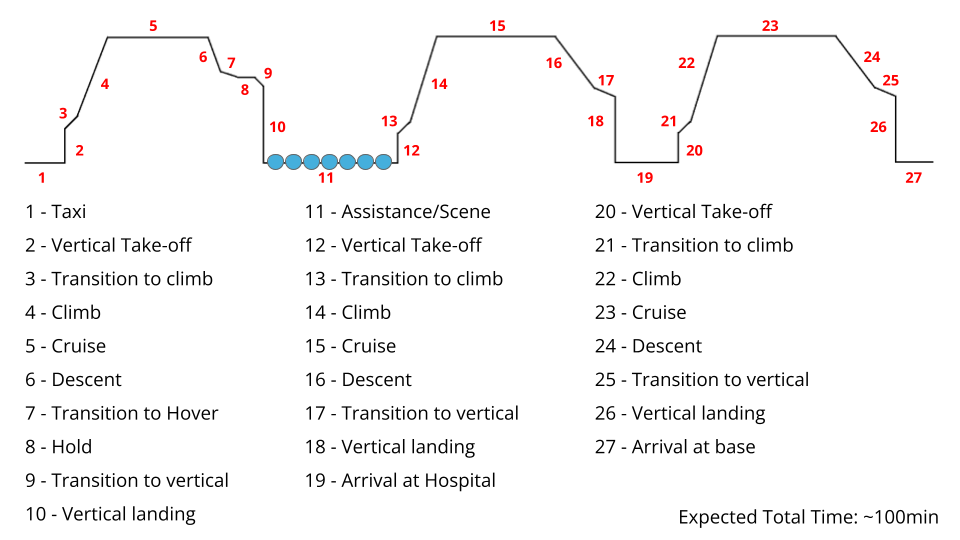
\includegraphics[width=\textwidth]{Imagens/PI - Semana 3.png}
    \caption{Missão}
    \label{fig:my_label}
\end{figure}
\FloatBarrier
O tempo foi estimado baseado em \textbf{who the fuck knows; inserir processo e citações}.\par
É importante mencionar que existe uma secção de Procura, secção 8, de forma a identificar o local onde a emergência toma lugar. Esta deverá ser entendida como voar a baixa altitude a menor velocidade do que aquela de cruise. É conceptualizada, também, como um voo com os rotores tilted com o ângulo de melhor eficiência. Este troço traz uma restrição ao design point (W/P, W/S) na forma de um teto máximo, sendo tanto maior quanto a velocidade. Foi entendido, duas semanas após esta, que o programa não conseguia simular esta manobra, devido à incapacidade de simular o forwards flight com tilted rotor, dando, por isso, uma restrição ao design space considerada excessiva e pouco realista.\par
{\Large{\textbf{Inserir aqui os dados todos deste json que estão no powerpoint}}}\par
As velocidades, os tempos e os ângulos foram estimadas baseado em {\large{\textbf{idfk,legit, fomos buscar isto onde}}}\par
\subsubsection{MTOW}
Para estimar o peso total da aeronave, foi tomados como dados históricos o peso do AW139, bem como o XV-15 {\large{\textbf{Imma be honest, eu não me lembro o que usamos como base, temos mesmo que ir ver}}}.\par
Dado, no entanto, o facto do programa discretizar a massa para cada componente, podemos usar apenas os dados antes mencionados para ter uma estimativa da massa total. Para obter a massa discretizada, foi necessário:
\begin{itemize}
    \item Estimar a massa de cada pessoa
    \item Estimar a massa do equipamento médico
    \item Estimar a proporção da massa de cada componente em relação à total
\end{itemize}
A massa de cada pessoa foi estimada em 100~kg, que é considerado uma estimativa conservativa e por cima. Foi baseado em {\large{\textbf{god knows where. and by god, I mean Joana, most likely}}}.\par
A massa do equipamento médico foi estimada com base em {\large{\textbf{god knows where. and by god, I mean Joana, most likely}}}.\par
A massa dos componentes da aeronave foi baseada no paper \cite{Bradley2015-yr}, em particular, na página 25, onde se encontra uma tabela, apresentada na figura \ref{sugartable}. Apesar de ser significamente diferente da nossa aeronave, foi considerado que era uma boa estimativa dos rácios de massa dum avião com configuração tube and wing, sendo por isso possível ajustar para o nosso design.\par
\FloatBarrier
\begin{figure}[h]
    \centering
    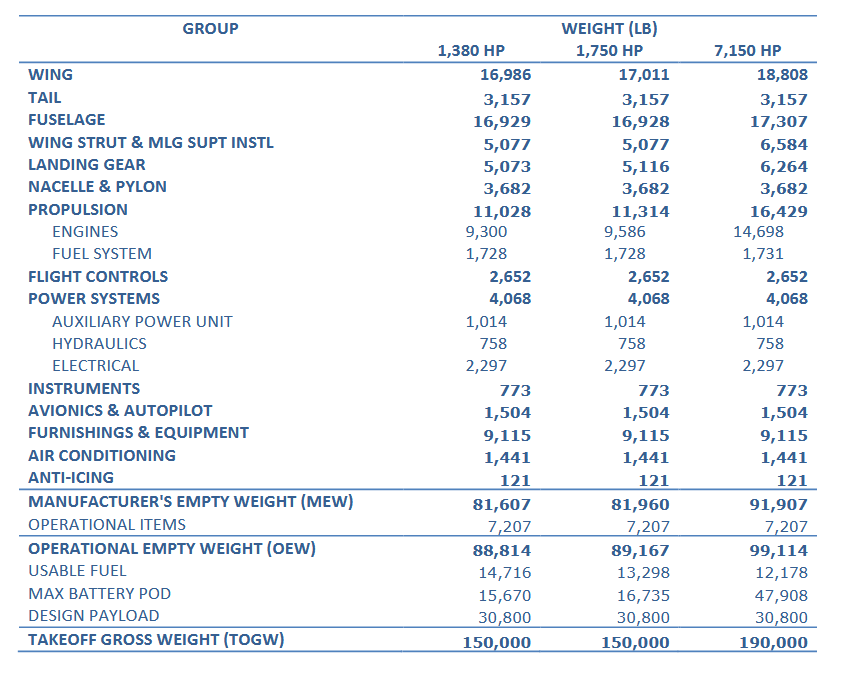
\includegraphics[width=\textwidth]{Imagens/boing sugar.PNG}
    \caption{Massa dos componentes do Boing SUGAR VOLT Source:\cite{Bradley2015-yr}}
    \label{sugartable}
\end{figure}
\FloatBarrier
Foi assumido uma relação linear, tal que a fração mássica fosse a mesma, ou aproximadamente igual, tanto no SUGAR VOLT como no nossa aeronave, no caso da estimação da massa das asas, cauda e fuselagem.\par
Dever-se-á notar que, nesta fase do projeto, não era sabido que o programa estimava o combustível e a massa das baterias, bem como que o VTOL era puramente a combustível. Devido a tal, foi estimada a massa de ambos baseado em dados históricos, nomeadamente, na percentagem da massa total que é do combustível.\textbf{Imma be honest, eu não sei onde fomos buscar os dados}\par
Abaixo, é apresentada a massa discretizada.\par
A altitude de cruise foi baseada na altitude mínima acima de zonas urbanas legislada pela FAA(?). \textbf{{\large{Quote, lol}}} Foi tido em conta que os helicópteros também conseguem voar a essa mesma altitutude \textbf{\large{{Quote, lol, AW139 deve ter uma altitude máxima de operaçao or something}}}
\FloatBarrier
\begin{table}[h]
\begin{tabular}{|l|l|}
\hline
Crew (100 kg/person)       & 200 kg                            \\ \hline
Passengers (100 kg/person) & 500 kg                            \\ \hline
Avionics                   & 24 kg                             \\ \hline
Payload Bay                & 200 kg (150 kg medical equipment) \\ \hline
Fuselage                   & 1200 kg                           \\ \hline
Main Wing                  & 840 kg                            \\ \hline
Horizontal Tail            & 100 kg                            \\ \hline
Vertical Tail              & 50 kg                             \\ \hline
Turboshaft -               & 462 kg                            \\ \hline
Battery                    & 200 kg                            \\ \hline
Generator                  & 462 kg                            \\ \hline
Electric Motor             & 510 kg                            \\ \hline
Fuel Tank                  & 1000 kg                           \\ \hline
\end{tabular}
\caption{Massa da aeronave discretizada - Semana 3}
\end{table}
\FloatBarrier
\subsubsection{Energy Network}
Tal como referido nas secções anteriores, foi escolhida uma arquitetura puramente turbo elétrica. Esta foi codificada no ficheiro json da seguinte forma:
\FloatBarrier
\begin{figure}[h]
    \centering
    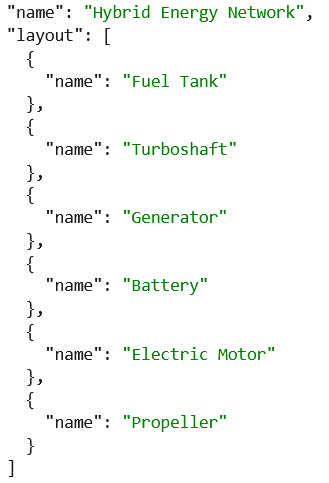
\includegraphics[width=0.4\textwidth]{Imagens/energy semana 3.png}
    \caption{Energy Network}
    \label{fig:my_label}
\end{figure}
\FloatBarrier
Esta configuração veio a ser considerada puramente conceptual devido a limitações do programa. A bateria teve que ser removida desta, posteriormente, devido ao facto do programa não simular recarregamento de baterias em voo. Também não era possível ligar a bateria e os motores elétricos em paralelo, dado que o programa só aceita arquiteturas sem ramos paralelos.\par